\subsection{CodeMirage}
\label{section:CodeMirage}
The work and dataset presented in the CodeMirage 
publication aim to evaluate ten LLM code detection 
methods. The dataset was also used to train the detectors 
(at least those requiring training).
They employed as many as ten different LLMs for 
code generation.

\begin{itemize}
    \item \textbf{GPT-4o-mini} \cite{openai_gpt4o_2024} : A proprietary model developed by OpenAI, selected to represent the state-of-the-art among large-scale, closed-source LLMs.
    \item \textbf{GPT-o3-mini} \cite{o3mini-openai-2025} : A smaller model from OpenAI's o3 series, known for high performance in STEM and logic benchmarks despite reduced parameter count.
    \item \textbf{Qwen-2.5-Coder-32B} \cite{hui2024qwen2} :  A specialized, code-centric LLM. Trained on high-quality multilingual code data, it supports over 40 programming languages and offers a 128K context window
    \item \textbf{Claude-3.5-Haiku} \cite{anthropic2024model} : The smallest member of Anthropic’s Claude 3.5 family
    \item \textbf{DeepSeek-R1} \cite{guo2025deepseek} : A reasoning-optimized model developed using reinforcement learning to enhance multi-step logical thinking.
    \item \textbf{DeepSeek-V3} \cite{liu2024deepseek} : A large-scale, general-purpose model from DeepSeek AI.
    \item \textbf{Gemini-2.0-Flash} \cite{google-gemini2-flash-2025} : Although designed for speed, it retains strong performance across code and reasoning tasks.
    \item \textbf{Gemini-2.0-Flash-Thinking} \cite{google-gemini2-flash-2025} : An experimental version of Flash that integrates internal “thinking steps” during generation. 
    \item \textbf{Gemini-2.0-Pro} \cite{google-gemini2-flash-2025} : The full-sized flagship model from the Gemini 2.0 series, comparable to GPT‑4 in overall performance.
    \item \textbf{Llama-3.3-70B} \cite{grattafiori2024llama} : A 70-billion-parameter open-source model from Meta AI, part of the LLaMA 3.3 release. It represents one of the most capable open LLMs available to the public.

\end{itemize}







\subsubsection*{Strengths}
\begin{itemize}
    \item The entire generation process is well documented; both 
    the Code Summarization methods 
    (necessary to obtain the prompts to be given to 
    the LLMs for generation) and the code 
    generation prompts are easily accessible 
    Figure~\ref{fig:propt_generation}. 
    {(\scriptsize\textit{Section 3:CodeMirage Framework})}
    \item The dataset also includes code samples with Paraphrasing, 
    meaning simulated modifications of small stylistic elements 
    in the code generated by LLMs.
    {(\scriptsize\textit{Section 3.1:Benchmark Construction})}
    \item The dataset, available on the official 
    \href{{https://huggingface.co/datasets/HanxiGuo/CodeMirage}}{huggingface} 
    portal is well documented.
    \item The dataset is perfective balanced.
\end{itemize}



\subsubsection*{Weaknesses}
\begin{itemize}
    \item The work itself explicitly requires the LLM-generated 
    code to match the length of the original human-written 
    code in the generation prompt, which is unrealistic and 
    disadvantages stylistic detection methods.
    {(\scriptsize\textit{Section 3.2:Benchmark Statistics})}
    \item All human-written code comes exclusively from the 
    \textbf{CodeParrot GitHub-Code-Clean dataset} 
    \cite{codeparrot-github-code-clean-2022}, 
    meaning that the dataset covers only a single domain.
    \item A comment-free version of the code is not provided, 
    which leads to some code samples being heavily 
    commented in a distinctly human style
    Figure~\ref{fig:code_example}. 
    It is not specified whether comments are removed prior to the 
    detection process; if not, many results could be 
    significantly biased.
    \item Although the paper does not explicitly highlight this, for each 
    human-written code sample, two LLM-generated versions are produced 
    rather than just one. This means that the actual ratio between human 
    and LLM-generated code is 1:20 Figure~\ref{fig:distribution}. 
\end{itemize}



\subsubsection*{Code Quality}
In order to preserve quality in the LLMs code source:
\begin{itemize}
    \item \textit{"consistency with the original human-written code's line count and character length"}
    \item \textit{"adequate token-level divergence from the original, enforced by requiring a 
    BLEU \cite{papineni2002bleu} score below 0.5 to avoid recitation."} 
\end{itemize}




%\begin{figure}[H]
%    \centering
%    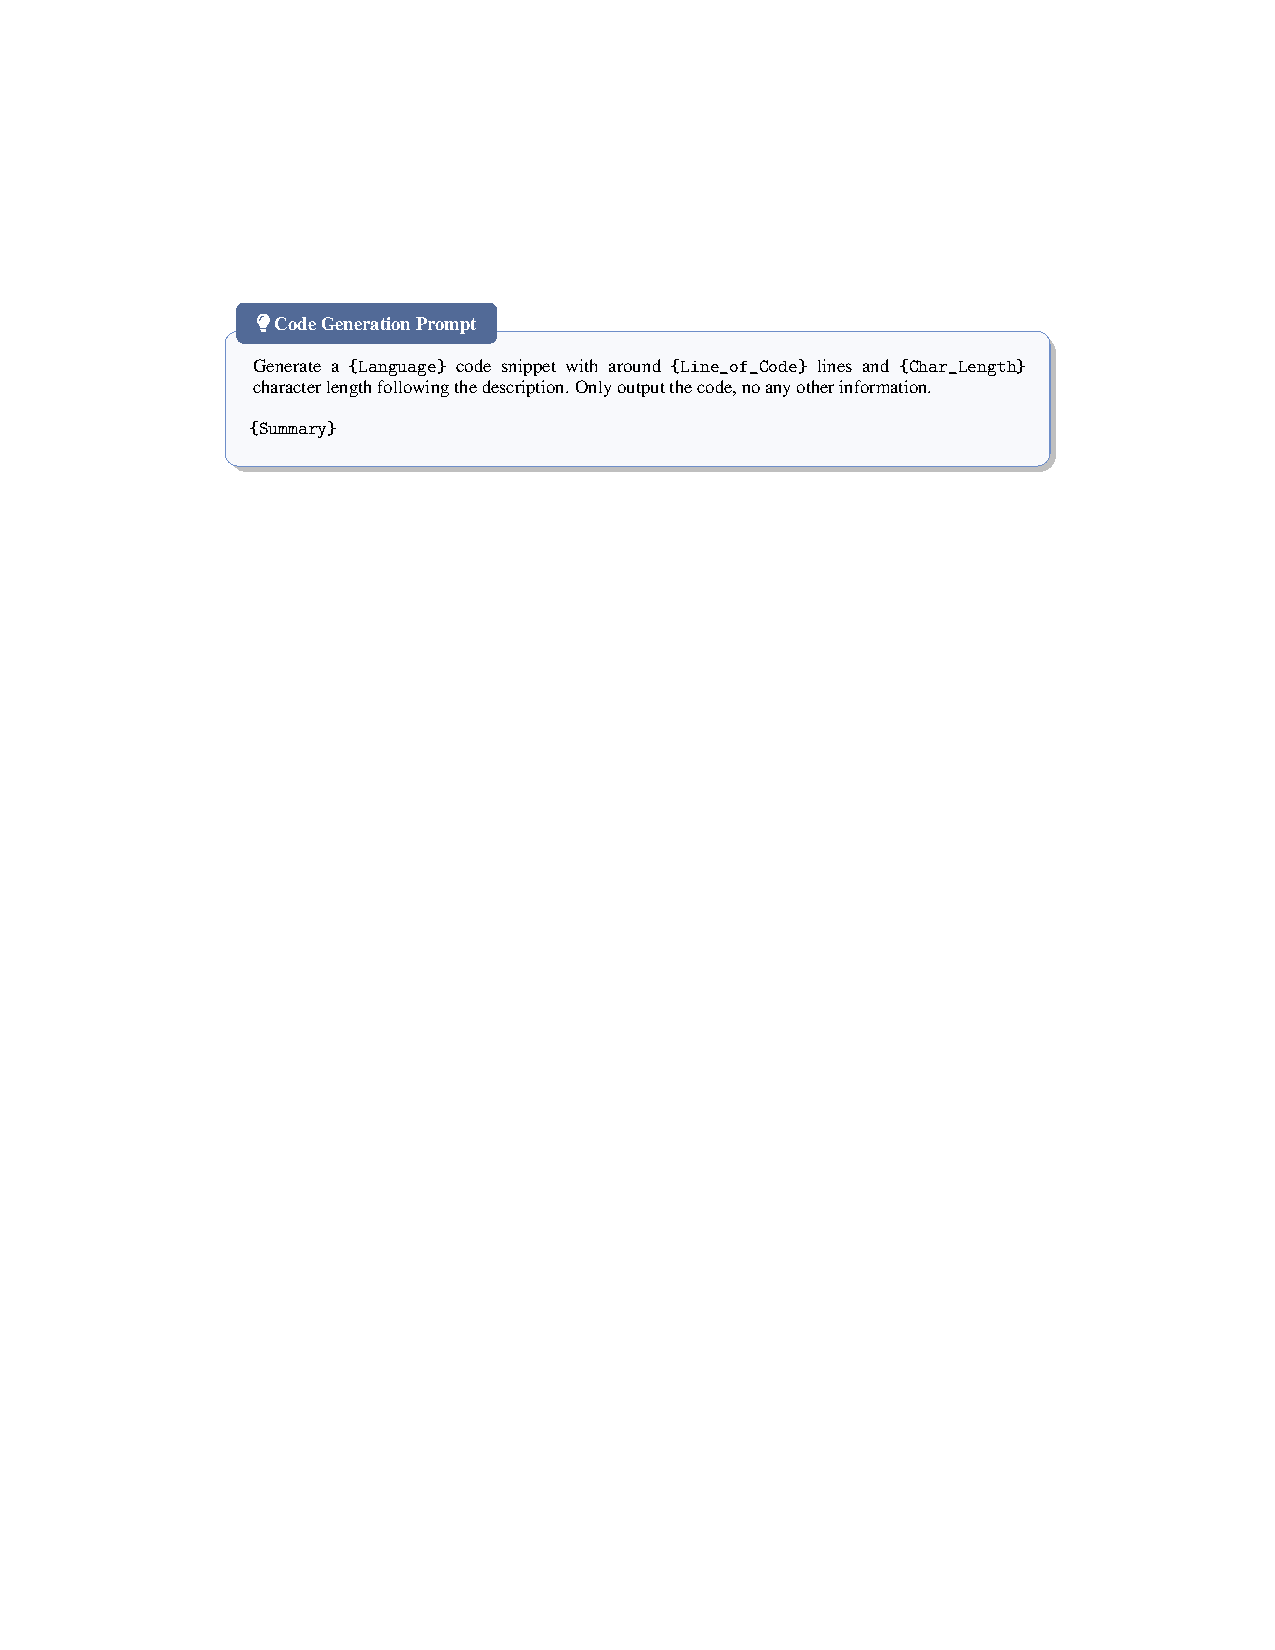
\includegraphics[width=0.6\textwidth]{img/CodeMirage/Propt_Generation.pdf}
%    \caption{Code generation prompt}
%    \label{fig:propt_generation}
%\end{figure}




\subsubsection*{Final evaluation}


\expandafter\def\csname CodeMirageHumanCode\endcsname{10,000}
\expandafter\def\csname CodeMirageLLMCode\endcsname{199,988}
\expandafter\def\csname CodeMirageNumLLMs\endcsname{10 LLMs: \textit{(GPT-4o-mini, GPT-o3-mini, Qwen-2.5-Coder-32B, Claude-3.5-Haiku, DeepSeek-R1, DeepSeek-V3,  Gemini-2.0-Flash,  Gemini-2.0-Flash-Thinking, Gemini-2.0-Pro, Llama-3.3-70B )}}
\expandafter\def\csname CodeMirageLLMDiversity\endcsname{6 different source models: \textit{(GPT, CodeQwen, Claude, DeepSeek, Gemini, Llama) }}
\expandafter\def\csname CodeMirageCurrentUse\endcsname{2024-2025}
\expandafter\def\csname CodeMirageLanguages\endcsname{\textit{(HTML, JavaScript, Java, C, Python, Ruby, Go, C\#, C++, PHP)}}
\expandafter\def\csname CodeMirageCodeTypes\endcsname{unspecified}
\expandafter\def\csname CodeMirageCodeSize\endcsname{1\textsuperscript{st} percentile: 639 words,\newline 3\textsuperscript{rd} percentile: 804  words}
\expandafter\def\csname CodeMirageCodeContext\endcsname{open-source}
\expandafter\def\csname CodeMiragePrompts\endcsname{Provided (one)}
\expandafter\def\csname CodeMirageSources\endcsname{GitHub}
\expandafter\def\csname CodeMirageCodeQuality\endcsname{Statistical alignment}
\expandafter\def\csname CodeMirageReliability\endcsname{Midium, \textit{(no precise references are provided regarding the data source)}}


\evaluationTable{CodeMirage}


Although the dataset appears to be well-varied and balanced, 
the lack of an evaluation of the actual functionality of the code 
may compromise the overall assessment. Furthermore, 
competitive-style code samples are completely absent.

\begin{figure}[H]
    \centering
    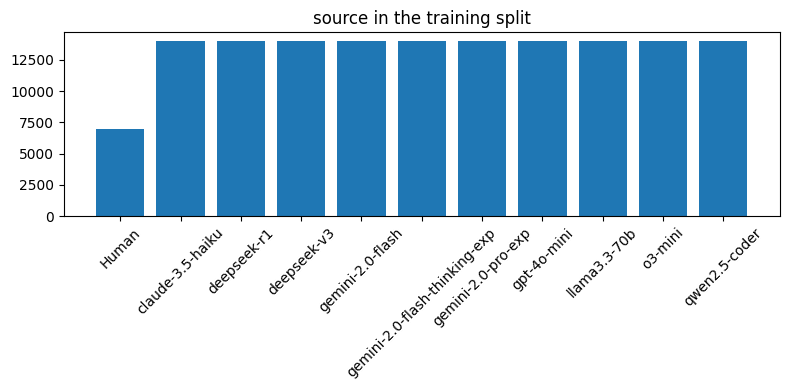
\includegraphics[width=0.8\textwidth]{img/CodeMirage/source.png}
    \caption{Source distribution}
    \label{fig:distribution}
\end{figure}